\graphicspath{{literature/fig/}}

\chapter{Literature}

\section{Sail Theory}
This section covers the sailing theory that is required for the sections that follow, and is taken from the official manual of the american sailing 
association\cite{ASA}. Fig. \ref{fig:sailboat_anatomy} illustrates the anatomy of a typical sailboat. The anatomy of a sailboat is as follows:

\begin{itemize}
    \item Hull: Watertight floating body of the sailboat that gives it form and supports all parts of the part.
    \item Keel: Fixed fin on the underside of the sailboat that provides sideways resistance needed to counter the force of the wind on the sails.
    \item Stern: The back-end of the sailboat.
    \item Bow: The front-end of the sailboat
    \item Starboard: When standing at the stern, facing the bow, starboard is the right side of the boat.
    \item Port: When standing at the stern, facing the bow, port is the left side of the boat 
    \item Rudder: Fin located beneath the stern. The angle of the rudder is adjusted to steer the direction of the sailboat.
    \item Helm: The mechanism by which the rudder angle is adjusted.
    \item Mast: Vertical beam attached to the hull which houses the mainsail
    \item Mainsail: Sail that attaches to the mast of the sailboat.
    \item Jib: sail that attaches to the bow and the top of the mast.
\end{itemize}

\begin{figure}[!h]
    \centering
    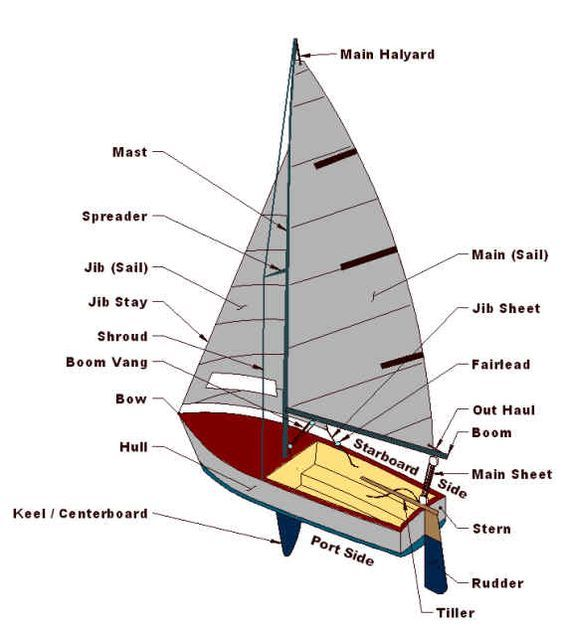
\includegraphics[width=0.6\linewidth]{sailboat_anatomy_1}
    \caption[Sailboat anatomy]{Sailboat anatomy \cite{sail_anatomy}}
    \label{fig:sailboat_anatomy}
\end{figure}

When on a sailboat the direction of the wind relative to the boat is known as the apparent wind, the direction of the wind relative to a fixed point - 
a point that has a zero velocity - is known as true wind. When the sailboat has a velocity that is not zero - sailboat not standing still - the apparent 
wind has a velocity that differs from the velocity of true wind. Fig. \ref{apparent_wind} illustrates this concept. 

\begin{figure}
    \centering
    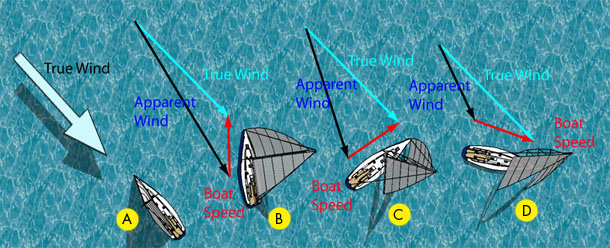
\includegraphics[width=0.7\linewidth]{apparent_wind.jpeg}
    \caption[Apparent wind]{Apparent wind\cite{apparent_wind} }
    \label{fig:apparent_wind}
\end{figure}


The sail of a sailboat acts similar to that of a airplane wing - it produces lift when orientated correctly. It is this lift that propels the sailboat 
forward. The orientation of the sail relative to the apparent wind therefore determines how much force is applied to the boat, any component of this force
that acts perpendicular to the centerline of the boat is canceled by the apposing force of the water on the keel. The act of changing the orientation of 
the sails is know as 'trimming the sails'. To generate a maximum amount of forward force on the sailboat, the sail must be positioned to capture as much 
of the winds energy as possible. The direction of apparent wind determines the directions that the sailboat can/cannot sail, these directions are known as 
points of sail and are measured relative to the direction of apparent wind. Fig. \ref{points_of_sail} illustrates the points of sail of a sailboat. It should 
be noted that there is a range known as the 'no-sail zone' in which a sailboat cannot sail. This range is measured $45^{\circ}$ to both sides of the apparent wind
when sailing directly towards the apparent wind.

\begin{figure}[!h]
    \centering
    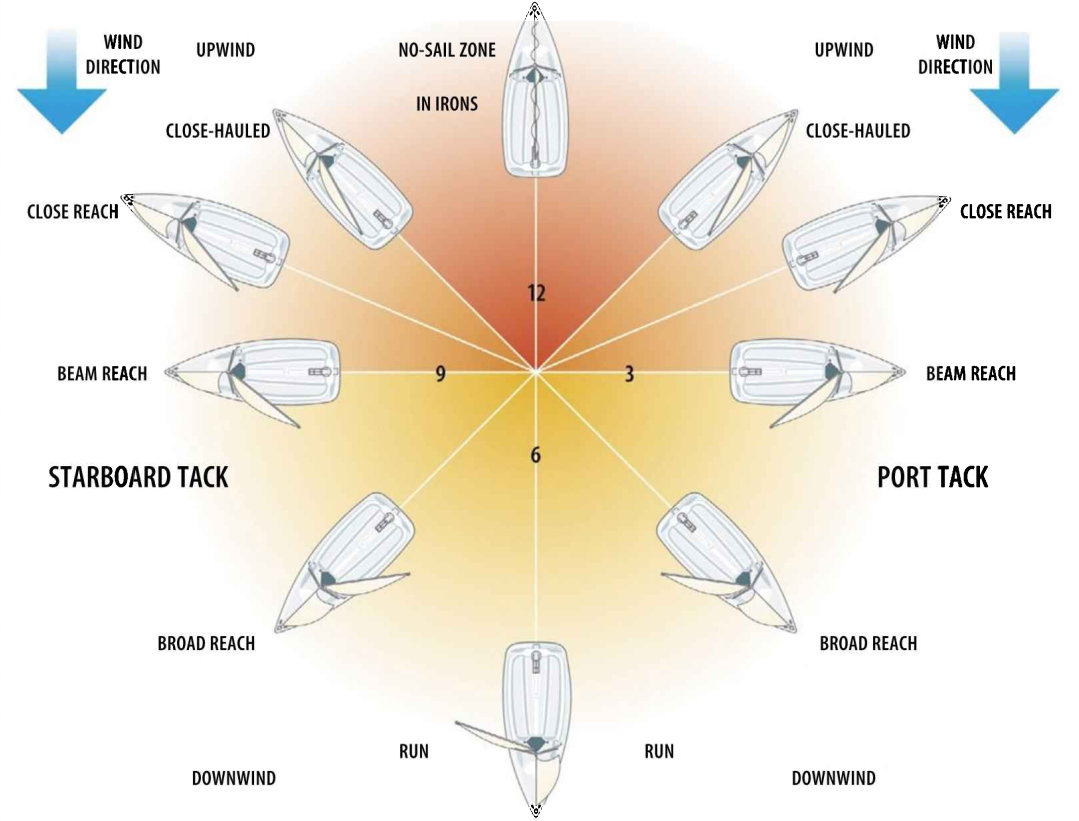
\includegraphics[width=0.7\linewidth]{point_of_sail.png}
    \caption[Point of sail]{Point of sail\cite{ASA} }
    \label{fig:point_of_sail}
\end{figure}

Point of sail is traditionally measured analogous to a clock, as shown in Fig. \ref{point_of_sail}. For the purpose of this report point of sail will be defined 
as the angle between apparent wind direction and the direction of travel of the boat, measured clockwise in degrees. A sail direction of $0^{\circ}$ will 
then correspond to 12'oclock in Fig.\ref{point_of_sail} and $180^{\circ}$ will corresponding to 6'oclock measured clockwise. The position of the mainsail will be 
defined by the angle between the mainsail and the centerline of the sailboat to either the starboard or port side.

If the desired destination is within the no-sail zone, a manoeuver known as 'tacking' can be performed to reach the desired destination. When sailing with 
he wind blowing on the starboard, its on the starboard tack, and when the wind is blowing on port side, the boat is on port tack. Tacking is the act of 
turning the bow of the sailboat through the no-sail zone. Assume the boat is on starboard tack and point of sail is $45^{\circ}$, after some distance has been travelled 
the bow is turned through the no-sail zone to attain a port tack and a point of sail of $-45^{\circ}$, this 'zig-zag' motion is done continuously until the 
desired destination is reached.

Another important manoeuver is the 'jibe', which is defined as the action of changing from a starboard tack to a port tack. An example of this occurring is when 
point of sail changes from $160^{\circ}$ to $100^{\circ}$, initially apparent wind will be port side but after crossing over $180^{\circ}$ the wind will be starboard side, 
during this crossover the mainsail will often swing from starboard to port.
\section{Related Work}

\subsection{Unmanned Sailing Vessel by Philip van Schalkwyk}
Philip is a mechatronics graduate who designed and developed an unmanned sailing vessel for his final year project at Stellenbosch University \cite{Phillip}.

\subsubsection{Objectives}
The purpose of the project was to design and develop an USV that is capable of semi-autonomous sailing. The objectives are as follows:

\begin{itemize}
    \item Design and develop a low-cost digital compass that produces accurate readings with tilt compensation.
    \item Design and develop a a low-cost mechanical wind vain that consists of a digital compass for wind direction sensing.
    \item Retrofit a RC sailing vessel with a micro-controller, digital compass, wind direction sensor, GPS unit and micro-SD card.
    \item Design and implement navigational and control systems to enable autonomous sailing.
\end{itemize}

\subsubsection{Method Used}
A RC sailing vessel was retrofitted with a micro-controller that would read data from sensors and adjust the rudder and sail position in order to sail along a 
desired path. The system consisted of a micro-controller, GPS receiver, a micro-SD card, an digital compass, wind direction sensor and two servo motors - one to control the 
sail and one to control the rudder angle. The micro-controller that was used was a Espress ESP-WROOM-32 micro-controller which is relatively low cost and has 
a 240 MHz clock speed. The electronic compass was used to determine the current bearing of the vessel, it was designed and developed using a magnetometer, 
accelerometer, gyroscope and tilt compensation algorithms. The MPU9250-6500 9-axis sensor module was used for the electronic compass as it consists of a magnetometer, accelerometer and a 
gyroscope. A mechanical wind vain was designed with CAD software and printed with a 3D printer. The wind vain
was fitted with a magnetometer - also the MPU9250-6500- which was used to determine the bearing of the wind vane and therefore the wind direction. The GPS receiver that was used for the navigational
system was a Neo M8N GPS, it would log positional data to the micro-SD card. 

A proportional controller was used to control the rudder position. The desired heading/bearing was calculated using the current GPS coordinates obtained from the 
GPS receiver and the target GPS coordinates. A sample would then be taken from the electronic compass which would give the current bearing of the vessel, the difference 
the current bearing and the desired bearing is the error signal. The proportional controller would then determine the rudder angle given this error signal, and the servo 
motor controlling the rudder would be adjusted accordingly. 

The main sail position was determined by the samples taken from the wind direction sensor and the current bearing. Only three point of sail classifications were used for the sail positions 
: close-hauled, beam-reach and run. This was done to give more time to navigational and rudder control systems. If it was determined that angle of attack was less than $45\deg$
the vessel would tack into the wind. This was achieved by calculating the bearing to either side of the no-sail zone, the vessel would then sail with one of these bearings for 50 meters 
and then change to the other bearing. The vessel would alternate along these bearings until the target destination was reached.

\subsubsection{Results}
The e-compass was tested against a magnetic compass and the results showed the average error in bearing to be $5.84^{\circ}$, the e-compass did however produce a consistent spike at $180^{\circ}$ across
multiple tests. Tests that were done with the GPS receiver showed that the positional accuracy of the GPS receiver was sufficient for the navigational system and data-logging. The wind sensor that
was developed was unable to provide wind direction data consistently, a possible explanation for this is that the length of the $I^{2}C$ connection is too long and therefore the capacitance in the lines caused 
a low pass filter effect on the signal. In the final tests that were conducted to verify the successful operation of the control systems, the point of sail classification was set to run initially and sail adjustments were not taken 
throughout the duration of the test - due to the wind sensor not working. The results of the final test showed that the rudder control system was capable of keeping the vessel on a near constant 
heading, with a maximum absolute error of $6\circ$. This test was conducted between two GPS coordinates and the vessel therefore sailed on a fixed bearing between them. Fig \ref{fig:phillip_lake_test} shows
the results of this final test.

\begin{figure}[!h]
    \centering
    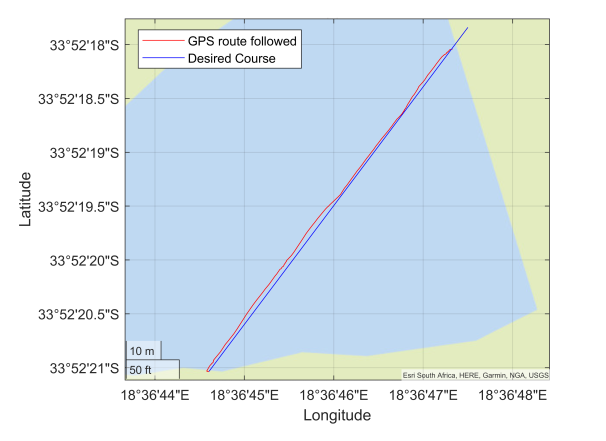
\includegraphics[width=0.918\linewidth]{phillip_lake_test}
    \caption[Test results from lake test]{Test results showing deviation of vessel from ideal trajectory \cite{Phillip}}
    \label{fig:phillip_lake_test}
\end{figure}

\subsubsection{Remaining challenges}
The rudder control system designed by Phillip was capable of accurately tracking a desired bearing during tests. Proportional integral control could not be implemented due to the consistent error that occurred during 
the e-compass testing. The USV that was developed does not however have the ability to dynamically adjust the sail position according to the relative wind direction, and is therefore unable to achieve the desired 
performance if wind direction is not constant. Tests where also not conducted to verify the tacking capabilities of USV.

\subsection{Design and Implementation of a Control System for a
Sailboat Robot}

\subsubsection{Objectives}
\begin{itemize}
    \item Determine the dynamic equations that govern the behavior of a sailboat.
    \item Use the dynamic equations to design - through simulation- a simple, however effective, controller that can be applied to different types of sail boats.
    \item Develop a prototype sailboat to implement and test a controller which was designed through simulation.
\end{itemize}

\subsubsection{Method Used}

The system that is developed for an autonomous sailboat consists of two processing units, a combination of sensors, and actuators/servos. Two processing units are used for a more 
flexible system. The one processing unit is a ATMega2560 which is built into an arduino, and is used to handle low level control decisions that should be executed in real time. 
The arduino communicates with the various sensors and implements the control algorithms used to control the actuators in a stable manner. The other processing unit is a Raspberry 
Pi which is responsible for high level navigation decisions, planning and external communication. The Raspberry Pi is connected to a base station via a XBee radio link of up to 1.6 Km. 
The two two processors communicate with each other via a RS-232 serial connection. The sensors that are used consist of a GPS receiver (EM-406 SiRF III), and a three axis digital compass 
(actual component used is not specified). A wind sock is used to determine wind direction and this is then transmitted to the system from the base station via XBee. Digital compass
is calibrated to compensate for local magnetic declination. 

The approach used to design an appropriate control system for an autonomous sailboat is to mathematically model the dynamics of the sailboat, and then through simulation, identify 
the optimal parameter values of the controller. Determining the dynamics that govern the behavior of a sailboat are divided into calculations of hydrodynamics, moment of inertia, 
viscous damping, lift, effort sail and centre of mass. These calculations are combined to form Eq. \ref{eq:sail_dynamics} which is used as the control law that governs sailboat control. 
In Eq. \ref{eq:sail_dynamics} $M_{a}$ refers to the hydrodynamics, $C_{rb}$ is dynamics(including centre of mass), $C_{a}$ refers to hydrodynamics related to coriolis and centripetal forces, 
$D_{k}$ term is the lift moments generated by the keel and $D_{h}$ are the lift forces acting on the hull.

\begin{equation}
    ( M_{RB} + M_{A} ) \dot{\upsilon} = \tau_{s} + \tau_{r} - (C_{RB}(\upsilon) + C_{A}(\upsilon))\upsilon  - (D_{k}(\upsilon) + D_{h}(V))V - g(\eta)
    \label{eq:sail_dynamics}
\end{equation}

Two controllers are initially developed: a PID controller for rudder control, and a fuzzy controller, which controls the sail position. By making use of Eq. \ref{eq:sail_dynamics} and simulation 
software (MATLAB) optimal parameter values are found for the PID controller. This approach is faster than the traditional method of adjusting the parameters, however since the 
mathematically model does not truly represent the sailboat the parameter values found are used as initial values to be further adjusted through experimentation.

The rudder controller takes in an error signal as its input and outputs the appropriate control signal to the rudder actuator. The error signal is determined as the difference 
between the actual bearing of the sail vessel and the desired bearing of the sail vessel. Desired bearing is calculated using current GPS location of the vessel and the target 
GPS location. The actual bearing of the sail boat is determined from the digital compass. 

The sail controller takes wind direction as its input and adjusts the sail position accordingly, the controller also takes into account limits of the sail vessel i.e. the dead-zone/no-sail zone.

In the sailboat prototype that is developed, the D parameter used in rudder control is disregarded, mainly because of instability, which is generated due to intensification 
of high-frequency noise caused by the derivative. 

\subsubsection{Results}

In the simulation the optimal gains for the rudder controller are: Kp = 0.68, Ki = 1.125 and Kd = − 0.130. These controller gains were used as initial values to be fine-tuned through
multiple tests done with the prototype sailboat. After conducting the tests the resulting adjusted rudder controller gains were: kp = 2.3 and ki = 0.8. The tests that were done 
compared the use of a proportional controller and a PI controller for the rudder control, Fig.\ref{fig:robotics_test_result} shows the results of one of the tests. Note that the 
sailboat was initially placed to face $90^{\circ}$ from target location. In all tests that were conducted the prototype sailboat reached the specified target coordinates, the PI 
controller, however, performed better than the P controller with less deviation from the ideal trajectory.

\begin{figure}[!h]
    \centering
    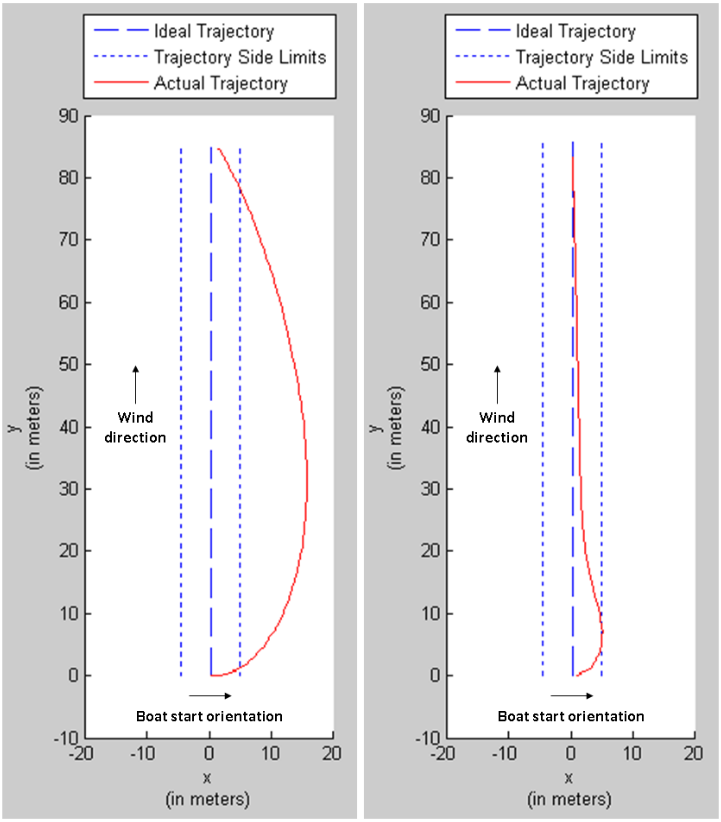
\includegraphics[width=0.6\linewidth]{robotics_test_result}
    \caption[Test results comparing P controller and PI controller]{Test results on water; P controller shown left and PI controller on right \cite{robotics5010005}}
    \label{fig:robotics_test_result}
\end{figure}

\subsubsection{Remaining challenges}

The system that was designed and developed does not incorporate an onboard wind direction sensor but instead receives the wind direction data from a base station via XBee. 
The sail vessel will therefore not be capable of travelling distances over which the apparent wind direction around the vessel differs from the wind direction around the base 
station. Aside from this, the system that was developed addresses the problem statement in section \ref{problem_statement}; the purpose of the following sections is then to duplicate the 
above system.


\subsection{FASt - An autonomous sailing platform for oceanographic missions}
the purpose of this project was to design and develope an autonomous sailing boat to enter the Microtransat competition - competition for fully autonomous sailing boats wherein the goal 
is to cross the atlantic ocean \cite{Alves2008FAStA}.

\subsubsection{Objectives}
\begin{itemize}
    \item Design and construct a high performance and light-weight sailboat of suitable size.
    \item Design and develope an electronics system that will enable long distance autonomous navigation and control of the sailboat.
    \item The electronics system must include a communication subsystem for short range and long range communication.
    \item The electronics system should have a low power consumption and powered by a power source that is recharged via photovoltaic cells.
\end{itemize}

\subsubsection{Method Used}
The sailboat hull shape was inspired by modern racing oceanic yachts and was constructed with fiber glass and epoxy resin. The total length of the sailboat is 2.5 m with a mast height 
of 3.4 m. It features two independently controlled rudders and two sails which are controlled simultaneously

The electronics system was divided into 5 subsystems: computing, communication, sensors, actuators and power management. The computing system consists of a 32-bit RISC microprocessor 
running with a maximum clock speed of 50 MHz, ROM memory which holds the bootstrap code and various digital modules that interface the processor with the sensors and actuators. The 
computing system was implemented using a FPGA, the one that was used was a Suzaki SZ130 which is built around a Xilinx FPGA. The board includes central Microblaze processor running
at 50 Mhz, 32 MB of SDRAM, 8 MB of SPI flash memory, a serial interface (RS232) and ethernet port implemented externally to the FPGA. The board has 86 input/output pins available,
which connect directly to the FPGA. The computing system runs uCLinux which a version of linux which has been simplified and adapted for embedded applications running processors 
with no memory management unit. The advantage of using an FPGA is that many of the processing and interfacing functions of the system can be implemented in custom hardware and 
therefore are not managed by a micro-processor; this allows the use of a micro-processor that runs at significantly lower clock speeds and thus lower overall power consumption.

The communications subsystem consists of a conventional WiFi router (LinkSys WRT54GC), a GSM modem (Siemens MC35), a IRIDIUM SBD modem (model 9601) and a radio control receiver. 
The WiFi router is to provide convenient short range communication with a laptop, mainly for the purpose of software development, debug and communication purposes. While at sea 
missions, the GSM modem and IRIDIUM SBD modem will enable small volume communications to take place. The GSM module enables communications within a range of a few kilometers from 
shore, the IRIDIUM SBD modem communicates via satellite connection and allows and therefore has a global range. The radio control receiver allows for manual control over the sailboat
 using a 4 channel proportional control RC transmitter.

Sensors used consist of a wind vane, anemometer, boom position sensor, digital compass (LinkSys WRT54GC), GPS receiver(uBlox RCB-4H), inclinometer, voltage monitors, ambient light 
sensor, interior temperature and a set of water sensors. The wind vain and boom position sensors were custom built using a magnetometer (Austria Micro Systems AS5040) and are used 
in the sail position control system. The anemometer is a conventional cup rotor that makes use of a hall effect switch, its main purpose is for data collection and data logging during 
sea missions. The digital compass and the GPS receiver are used for navigation and data logging purposes. The inclinometer is used to determine heel angle which is used to reef the sails. 
It should be noted that the sailboat that was developed does not have the ability to adjust the area of the sail i.e. reef, the inclinometer was included for future iterations of the 
project that possess have this ability. The voltage monitors are used to monitor the voltage of the batteries. The ambient light sensor is used to monitor light intensity which affects
 the voltage produces by photovoltaic cells. Specific hardware was designed and implemented in the FPGA to interface these sensors with the RISC micro-processor.

The actuators in the system consist of two standard high-power RC servos which provide independent control of the two rudders. The two sails are both controlled simultaneously by a 
DC geared motor. Although having a low efficiency the DC geared motor is extremely robust, and once position and un-powered the gearbox locks the motors shaft in place. Traditional 
servo motors consume power in holding a certain shaft position in response to an applied force on the shaft. The use of the DC geared motor is therefore advantageous as sail position
is only adjusted when changing course or if a change in wind direction occurs, therefore no power is consumed in keeping the shaft fixed in reaction to the force applied by the wind. 
A multiplexer was implemented in hardware to select the source data that is routed to the actuators, if a RC connection is established then this data is selected, otherwise data from 
the computing system is selected.
 
The power management system consists of a 45 Wp solar panel (Solara SM160M), two 95 Wh Li-ion batteries, a battery charging circuit and a highly efficient power supply. A wind generator
was considered to compliment the photovoltaic cells but ones available commercially are too large and heavy for this application. The total power consumption of the system was measured
to be 560 ma.

The software is divided into five modules that implement the five main tasks: hardware interface, helm, sail, skipper and logger. The hardware interface implements all the driver 
software needed for the processor to communicate with sensors,actuators and configuration parameters. The helm implements the PI controller used to control the rudder position according
 to wind direction and desired bearing. The commands supported by this module include keeping a fixed bearing, maintaining the angle of apparent wind and performing tacking or gibing 
 maneuvers. The sail module is responsible for controlling the sail position according to wind speed and direction and a set of rules that define best sail angle. This module also implements 
 reefing of the sails - the sheet is eased when heel angle is greater that a certain value. The skipper module sends commands to the helm and sail modules and is responsible for higher
  level navigation such as deciding what course to follow and when to perform certain sailing maneuvers. The logger module listens to all the other modules and stores relevant data in a log file.

\subsubsection{Results}
This article does not cover the testing of the system described above and therefore the validity of the design cannot be verified. The article does however highlight important hardware 
and software design features to consider when attempting to design an autonomous sailing vessel

\subsubsection{Remaining challenges}

The system made use of an FPGA to implement the central computing system as well as interface with the sensors and actuators of the system. While this
 does decrease the power consumption of the system it also greatly increases the complexity of the design. Many modern micro-controllers already incorporate the hardware needed to 
 interface with the various sensors and actuators used in this system. 

Given that the scope of this project stated in section \ref{}, low power consumption of the system, although important in long distance sea missions, is not of vital importance for 
the purpose of designing and developing the navigational and control systems for an autonomous sail vessel. 

The system included functionality that is not needed for the purpose of this project. Some of this functionality includes the simultaneous 
control of two sails, two rudder servo's, boom position sensing, wind speed sensing, heel angle sensing, a power supply that incorporates rechargeability and photovoltaic cells, and a 
communications subsystem for short and long range communication with the vessel.

\subsection{Establishing frame of reference}
\label{sec:reference_frame}

It is important to establish a fixed frame of reference which can be used to determine the orientation of a vessel at sea. The fixed frame of reference that will be used in this report 
is the industry standard "NED" (North, East, Down) coordinate system. The NED coordinate system is orientated such that at any position on the earth the x-axis is aligned with true north, 
the y-axis is aligned with lines of latitude and points east, the z-axis is aligned with the vector that represents the acceleration of gravity. The x,y-plane is therefore tangent to the 
sphere of the earth. The inertial frame of the sailing vessel is fixed to the body of the sailing vessel and is the perspective that a person on the sailing vessel would have. The x-axis of 
the inertial frame of the sailing vessel is aligned with the centerline of the vessel and points from the stern to the bow, the y-axis is aligned perpendicular to the centerline of the vessel
and points to the starboard side, the z-axis is aligned with the mast of the vessel and points downwards. This concept is illustrated in Fig. \ref{fig:reference_frame}. 

\begin{figure}[!h]
    \centering
    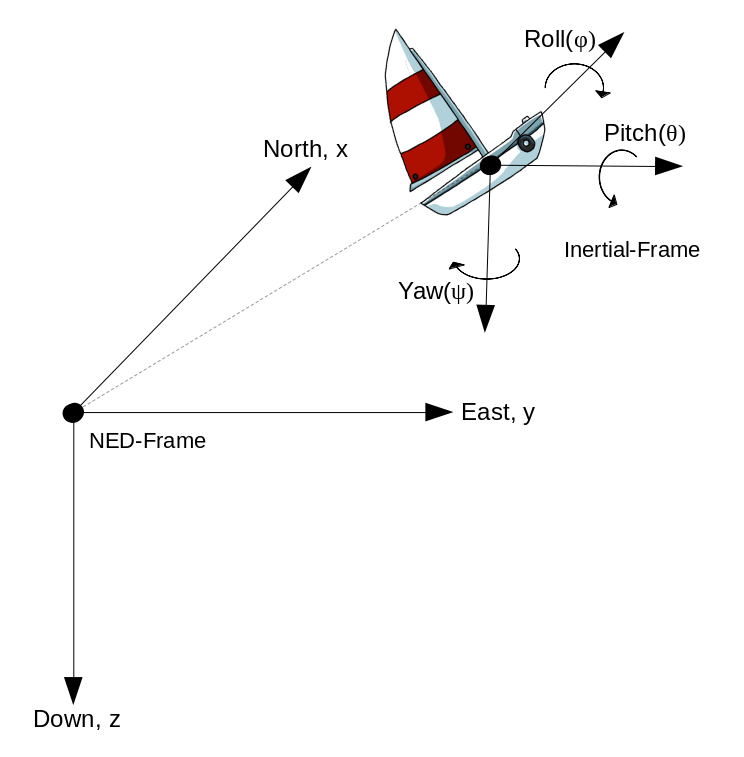
\includegraphics[width=0.5\linewidth]{reference-frame.png}
    \caption[NED frame of reference]{NED frame of reference}
    \label{fig:reference_frame}
\end{figure}

Rotation of the inertial frame about the x-axis is known as the roll angle ($\phi$), rotation about the y-axis is the pitch angle ($\theta$), and rotation about the z-axis is the yaw angle 
($\psi$). For all axes, clockwise rotation is taken to be positive rotation. Given that the roll, pitch, and yaw angles are all known it is possible to transform the inertial frame back to 
the NED frame using transformation matrices in Eq. \ref{eq:R_x}, \ref{eq:R_y}, \ref{eq:R_z} \cite{e_compass}. 

\begin{equation}
    \vec{R_{x,\phi}} = \begin{bmatrix} 1 & 0 & 0 \\ 0 & \cos\phi & -\sin\phi \\ 0 & \sin\phi & \cos\phi \end{bmatrix}
    \label{eq:R_x}
\end{equation}

\begin{equation}
    \vec{R_{y,\theta}} = \begin{bmatrix} \cos\theta & 0 & \sin\theta \\ 0 & 1 & 0 \\ -\sin\theta & 0 & \cos\theta \end{bmatrix}
    \label{eq:R_y}
\end{equation}

\begin{equation}
    \vec{R_{z,\psi}} = \begin{bmatrix} \cos\psi & -\sin\psi & 0 \\ \sin\psi & \cos\psi & 0 \\ 0 & 0 & 1 \end{bmatrix}
    \label{eq:R_z}
\end{equation}

\subsection{Magnetic declination}

A traditional handheld magnetic compass will align itself with the earths local magnetic field lines, which in theory run from the magnetic south pole to the magnetic north pole. This 
means that a magnetic compass will point to magnetic north. However in practice this is not true, the earths magnetic field lines are not constant, and depending on where measurements
are taken there will exist an angle of error. True north is defined as  

True north, also known as geographical north, is defined as the point where all lines of longitude intersect. Magnetic north is the point to which a magnetic compass aligns itself, and 
varies across the globe as well as with time. The direction of magnetic north differs depending location because earths magnetic field lines do not travel a linear path from magnetic 
south to magnetic north, this is illustrated in Fig. \ref{mag_declination}. 

\begin{figure}[!h]
    \centering
    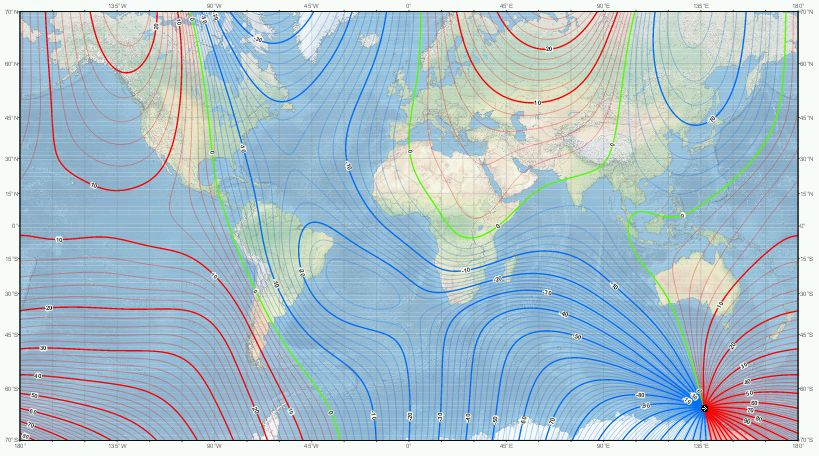
\includegraphics[width=0.9\linewidth]{mag_declination}
    \caption[Magnetic declination across the globe]{Magnetic declination across the globe \cite{Mag_declination}}
    \label{fig:mag_declination}
\end{figure}


Magnetic declination is an angle of correction used to determine true north from a local magnetic north reading. Magnetic declination takes into account the variance of local magnetic 
field lines and the angle between magnetic north and true north. Magnetic declination therefore differs across the globe. The National Oceanic and Atmospheric Administration (NOAA) \
keeps track of magnetic declination across the globe as it changes with time. The magnetic declination in Stellenbosch is $25.77^{\circ} \pm 0.59^{\circ}$.   